\documentclass{standalone}
\usepackage[T1]{fontenc}
\usepackage[utf8]{inputenc}
\usepackage{pgf,tikz}
\usepackage{setspace}
\usepackage{pgfplots}
\pgfplotsset{compat=1.12}

\begin{document}

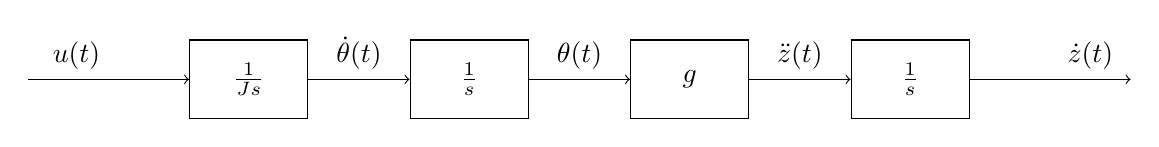
\begin{tikzpicture}[scale=1]
     \begin{scope}[yshift=-1.8cm, xshift=-7cm, node distance=28mm, block/.style={rectangle, draw, minimum width=15mm, minimum height=10mm}, sumnode/.style={circle, draw, inner sep=2pt}]
	 \node[coordinate] (input) {};
	 \node[block, right of=input,] (int1)  {$\frac{1}{Js}$};
	 \node[block, right of=int1, ] (int2)  {$\frac{1}{s}$};
	 \node[block, right of=int2, ] (gain)  {$g$};
	 \node[block, right of=gain, ] (int3)  {$\frac{1}{s}$};
	 \node[coordinate, right of=int3] (output) {};

	 \draw[->] (input) -- node[above, pos=0.3] {$u(t)$} (int1);
	 \draw[->] (int1) -- node[above] {$\dot{\theta}(t)$} (int2);
	 \draw[->] (int2) -- node[above] {$\theta(t)$} (gain);
	 \draw[->] (gain) -- node[above] {$\ddot{z}(t)$} (int3);
	 \draw[->] (int3) -- node[above, near end] {$\dot{z}(t)$} (output);
       \end{scope}
     \end{tikzpicture}
   \end{document}
   